%\documentclass[compress,t,11pt]{beamer}
\documentclass[handout,compress,t,11pt]{beamer}
\usetheme[]{metropolis}           % Use metropolis theme
\usefonttheme{serif}
\definecolor[named]{Gray}{RGB}{111,112,114}
\definecolor[named]{DarkGray}{RGB}{48,48,48}
\definecolor[named]{Cardinal}{RGB}{179,22,34}
\usepackage[T1]{fontenc}
\usepackage[altbullet]{lucidabr}
\usepackage{textcomp}
\usepackage{upquote} % needed to make straight quotes work in listings
\usepackage{listgolang}
\usepackage{mathtools}
\usepackage{comment}
\usepackage{tikz}
\usepackage{tikzsymbols}
 \usetikzlibrary{trees,shapes,plotmarks,arrows,er,automata,petri,topaths,positioning}
\usepackage{pifont}
\usepackage{clrscode}
\usepackage{setspace}
\usepackage{soul}
\usepackage{hyperref}
\usepackage{animate}

\setbeamercolor{palette primary}{fg=white,bg=Cardinal}
\setbeamercolor{palette secondary}{fg=white,bg=Gray}
\setbeamercolor{palette tertiary}{fg=white,bg=Cardinal}
\setbeamercolor{palette quaternary}{fg=white,bg=Gray}
\setbeamercolor{palette sidebar primary}{fg=white,bg=Cardinal}
\setbeamercolor{palette sidebar secondary}{fg=white,bg=Gray}
\setbeamercolor*{titlelike}{fg=Cardinal}
\setbeamercolor{structure}{fg=Gray}
\setbeamercolor{title separator}{fg=Cardinal}
\setbeamercolor{alerted text}{fg=Cardinal}
\setbeamercolor{reversed}{fg=Cardinal,bg=black}

\newcommand{\card}[1]{\ensuremath{\left|#1\right|}}
\newcommand{\norm}[1]{\ensuremath{\|#1\|}}

\title[Programming in Go]{\bf Programming in Go\\ Lesson 1: The Basics}
\author{Matt Holiday} 
\institute[CP]{Cardinal Peak}
\date{16 April 2019} 
%\titlegraphic{\hfill
\includegraphics[width=.25\textwidth,height=.25\textheight]{cp-logo-2x.png}}
\titlegraphic{
\begin{tikzpicture}[overlay, remember picture,scale=0.4]
\node[at=(current page.north east), anchor=north east] (a) {};
\node[below left = 0.1cm and 0.1cm of a] (b)
{
\includegraphics[width=.25\textwidth,height=.25\textheight]{cp-logo-2x.png}};
\node[below left=2.56cm and 2.9cm of b]
{
\includegraphics[width=.1\textwidth]{go-logo.png}};
\end{tikzpicture}}

\setbeamerfont{footline}{series=\bfseries\selectfont}
\setbeamersize{text margin left=12pt,text margin right=12pt}
\linespread{1.0}
\metroset{block=fill}

\hypersetup{
    colorlinks=true,
    linkcolor=Cardinal,
    filecolor=magenta,      
    urlcolor=blue,
}

\begin{document}
\frame{\titlepage} 

%\section{Introduction}
\begin{frame}[fragile]
    \frametitle{Lesson \# 1}
    What we'll cover today:
    \begin{itemize}
    \item Installation
    \item Running a simple program
    \item Simple types
    \item Declarations
    \item Initialization
    \item Assignment \& type conversion
    \item Reference types
    \item Basic control structures
    \item Standard I/O \& simple formatting
    \end{itemize}
\end{frame}

\begin{frame}[fragile]
    \frametitle{The Book}
    Hereinafter referred to as {\em GOPL} \par
    \vspace{0.4\baselineskip}
    \begin{minipage}[c]{0.55\textwidth}
        I will be taking exercise material 
        from this book \par
        \vspace{\baselineskip}
        
    Amazon paper: \$28 \par
    \vspace{\baselineskip}
    \verb|informit.com| PDF: \$19 \\
    (with coupon \verb|IUGD45|)
    \end{minipage}%
    \begin{minipage}[c]{0.35\textwidth}
        \vspace{0.5\baselineskip}
        \hfill 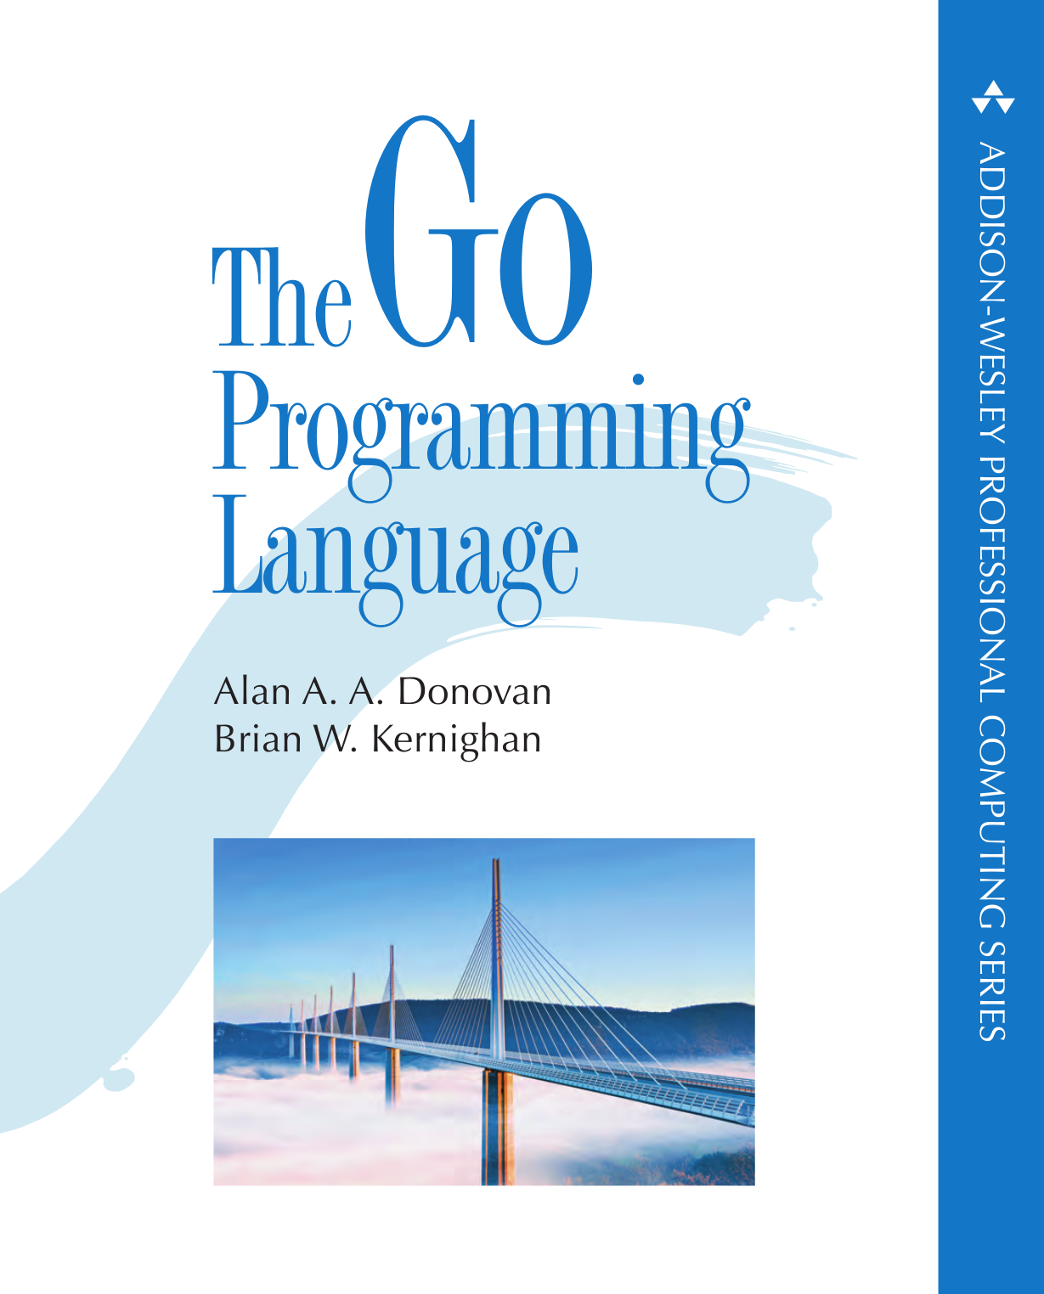
\includegraphics[width=0.85\textwidth,height=.5\textheight]{cover}
    \end{minipage} \par
    \vspace{2\baselineskip}
    ``Anything with Brian Kernighan's name on it is worth reading.'' \\--- Matt Holiday
\end{frame}

\begin{frame}[fragile]
    \frametitle{Installation}
    Start from the Go language page: \href{https://golang.org}{https://golang.org} \par
    \vspace{0.5\baselineskip}
    {\bf Mac}: run \verb|brew install go| (or use the installer package) \par
    {\scriptsize Homebrew installation: \href{https://brew.sh}{https://brew.sh}} \par
    \vspace{0.75\baselineskip}
    {\bf Windows}: open the installer (MSI) file and follow the prompts to install the Go tools \par
    {\scriptsize(otherwise you can download a ZIP file, but you have to set some environment stuff)} \par
    \vspace{0.75\baselineskip}
    {\bf Linux}: download the archive and extract it into \verb|/usr/local|, \\
    creating a Go tree in \verb|/usr/local/go| \\
    \vspace{0.5\baselineskip}
    {\scriptsize\verb|sudo tar -C /usr/local -xzf go1.12.4.linux-amd64.tar.gz|} \\
    \vspace{0.5\baselineskip}
    and don't forget to add \verb|/usr/local/go/bin| to \verb|$PATH| (Linux)\\
\end{frame}

\begin{frame}[fragile]
    \frametitle{GOPATH environment variable}
    If you work out of \verb|$HOME/go/src| you don't need to set it \par
    \vspace{0.5\baselineskip}
    Otherwise for what we're doing in class you'll need it \par
    \vspace{2\baselineskip}    
    The \href{https://golang.org/cmd/go/}{Go command} page tells you more than you want to know
\end{frame}

\begin{frame}[fragile]
\frametitle{Hello, world!}
What the simplest program looks like:
\begin{golang}
package main

import "fmt"

func main() {
    fmt.Println("Hello, world!")
}
\end{golang}
\end{frame}

\begin{frame}[fragile]
    \frametitle{Running a program}
    From the command line: \par
    \vspace{\baselineskip}
\begin{verbatim}
$ go run hello.go
Hello, world!

$ go run sieve.go 49
15: [2 3 5 7 11 13 17 19 23 29 31 37 41 43 47] 
\end{verbatim}\par
    \vspace{3\baselineskip}
    Later we'll talk about how to build binaries that stick around
\end{frame}

\begin{frame}[fragile]
\frametitle{Hello, playground!}
Simple programs run at the \href{https://play.golang.org}{Go playground}
    \vspace{-0.4\baselineskip}
\begin{center}
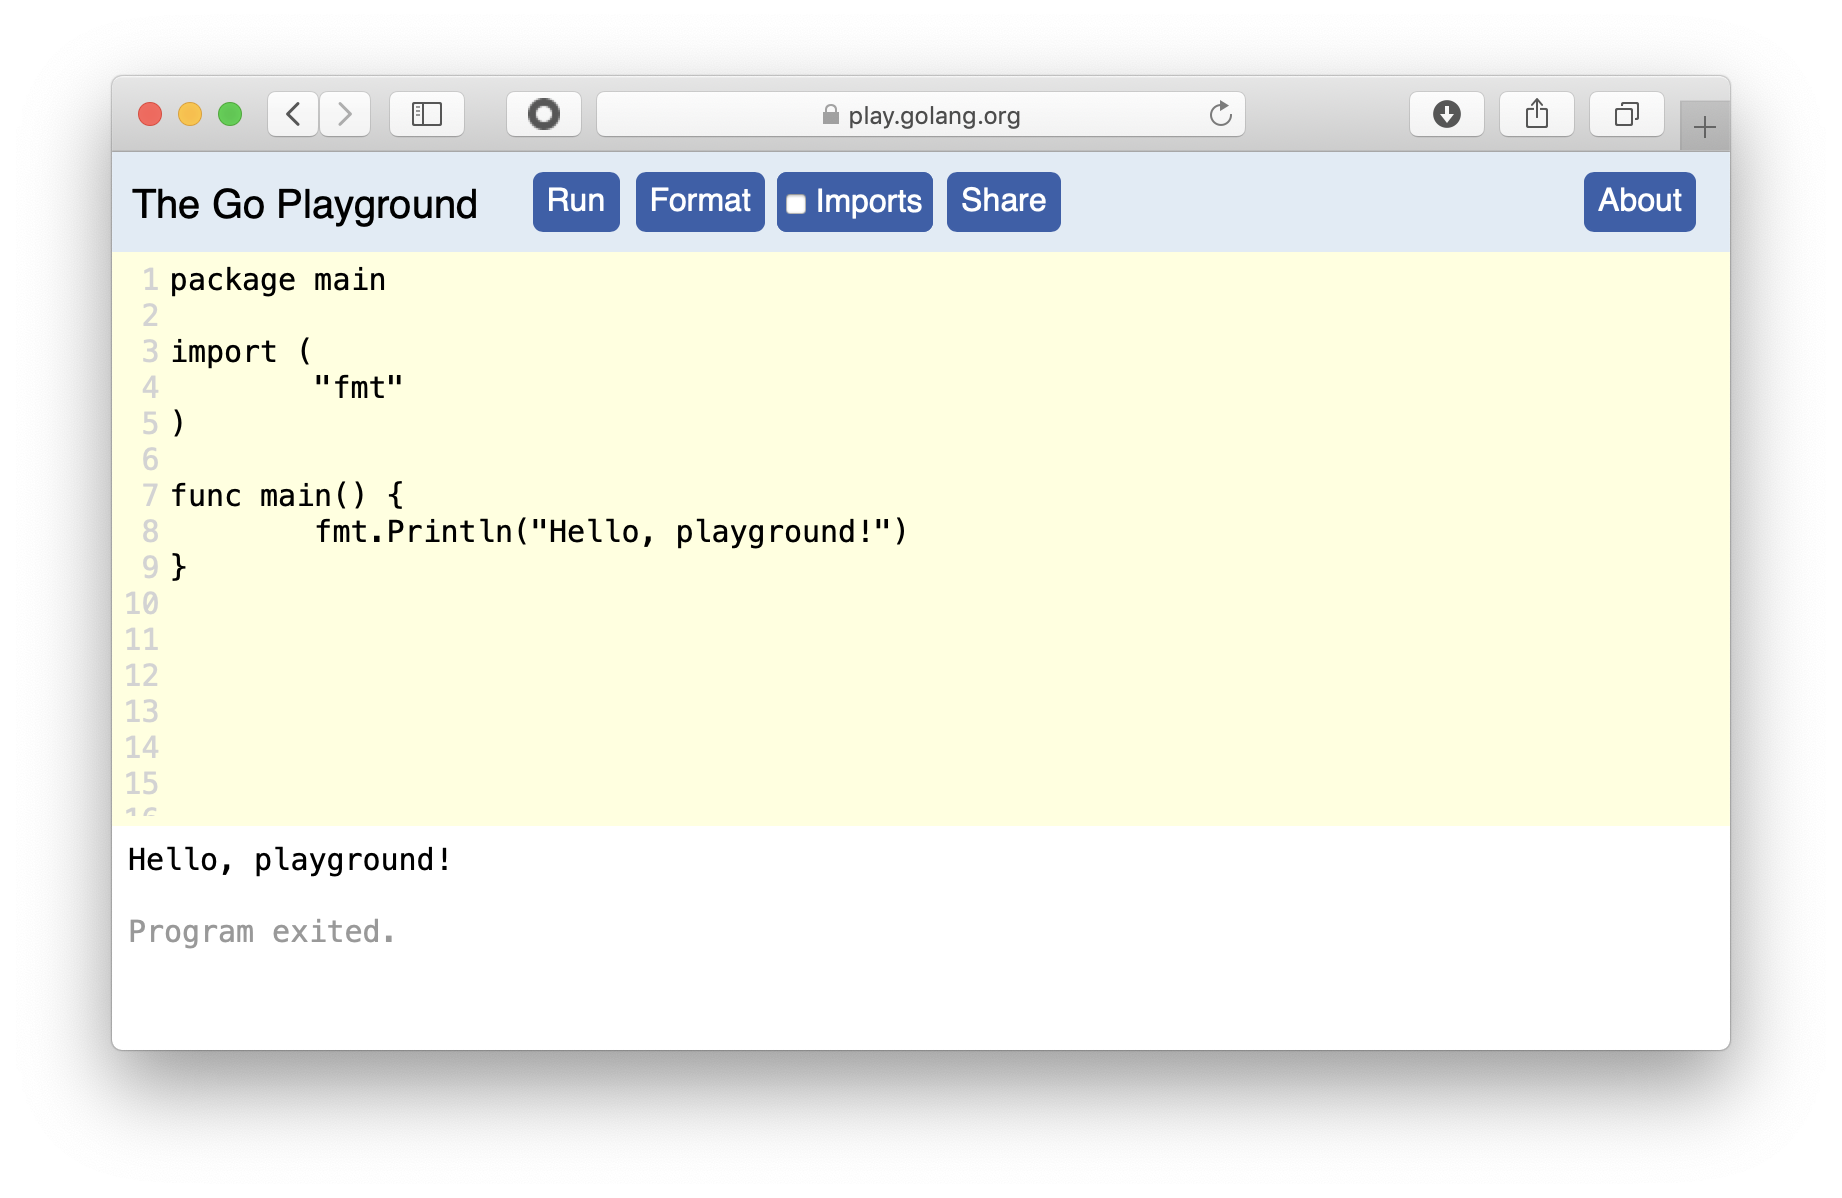
\includegraphics[height=.9\textheight]{go-playground.png}
\end{center}
\end{frame}

\begin{frame}[fragile]
\frametitle{More information}
Get all the info at \href{https://golang.org/doc/}{https://golang.org/doc/}
    \vspace{-0.6\baselineskip}
\begin{center}
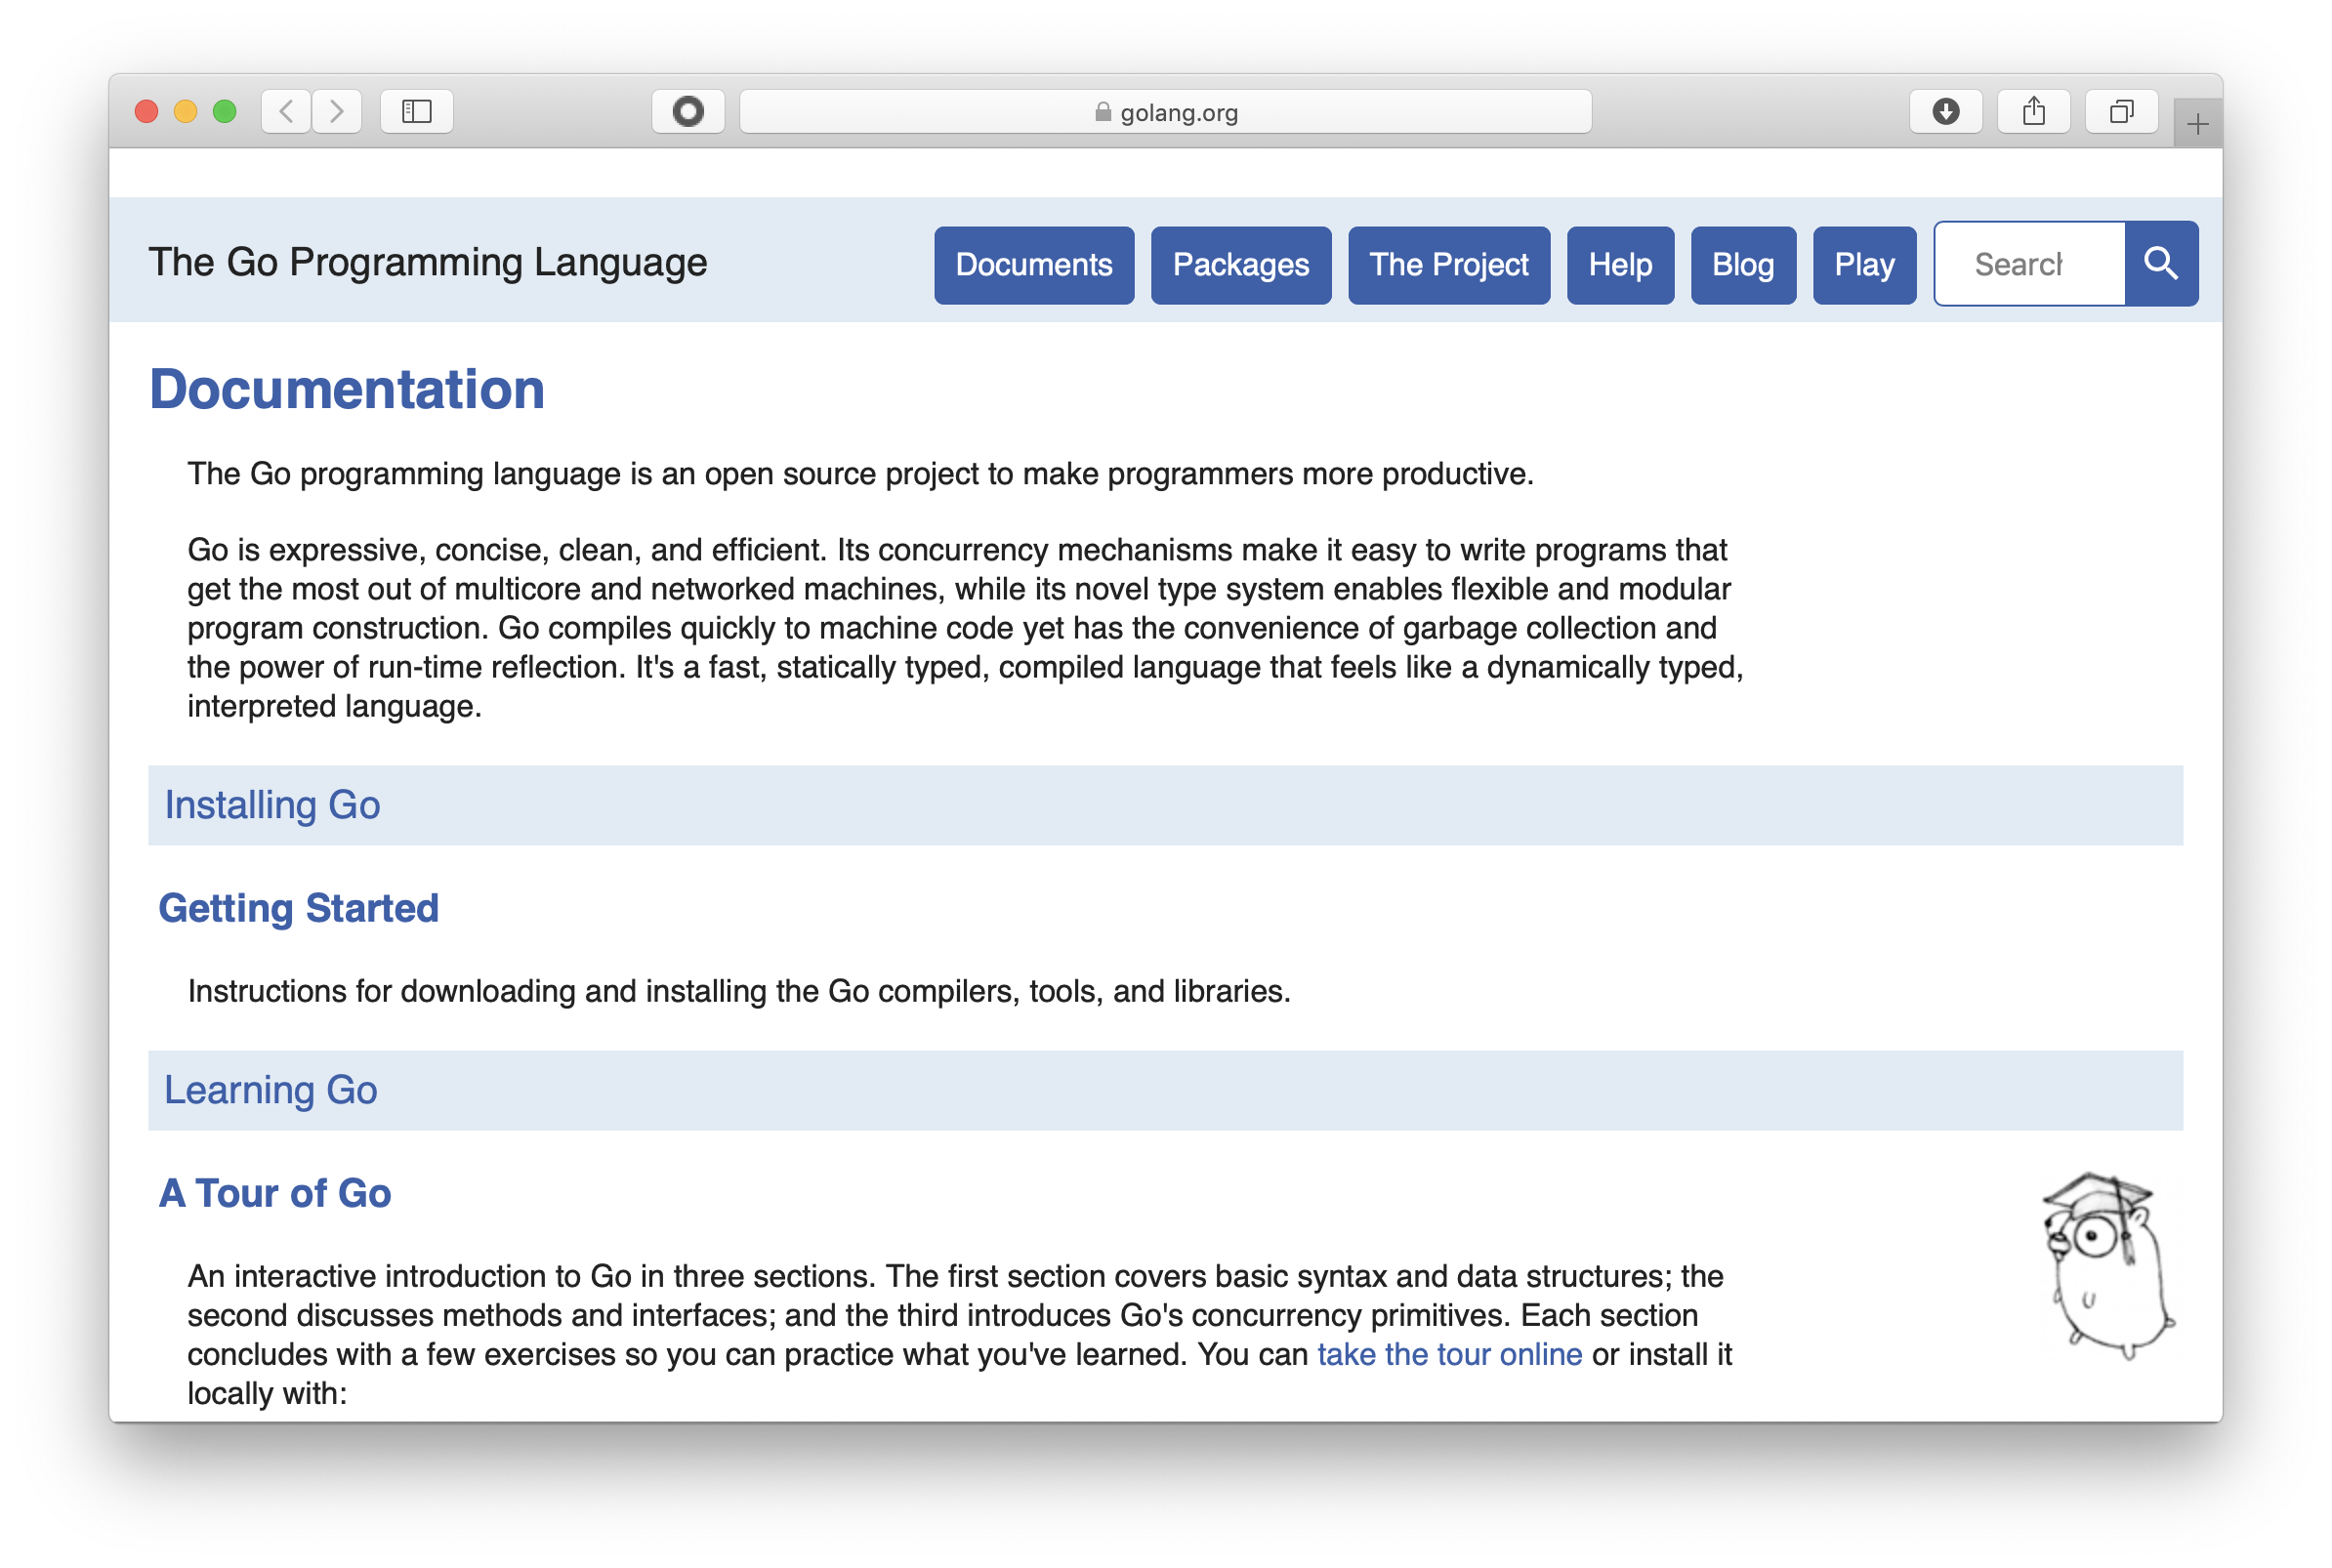
\includegraphics[height=.9\textheight]{golang-site.png}
\end{center}
\end{frame}

\begin{frame}{Something more complicated}
\begin{center}
\animategraphics[width=0.7\linewidth]{10}{erat/eratosthenes-}{0}{158}
\end{center}
\end{frame}

\begin{frame}[fragile]
\frametitle{Something more complicated}
\begin{golang}
package main

import "fmt"

// Find primes in the range 2..n and return them in a slice

func sieveOfEratosthenes(n int) []int {
    // Create a boolean array [0..n] as all true, and then
    // set entries false as they are found not to be prime

	integers := make([]bool, n+1) // why "n+1" and not "n"?

	for i := range integers {
		integers[i] = true
	}

    integers[0], integers[1] = false, false
\end{golang}
\end{frame}

\begin{frame}[fragile]
\frametitle{Something more complicated}
\begin{golang}
    // We "cross out" multiples of each prime because they
    // are divisible by that prime number; e.g., when p =
    // 2 we remove 4, 6, 8, ... and when p = 3  we remove
    // 9, 12, 15, ... and skip 6 because 6 = 2*3 was seen

	for p := 2; p*p <= n; p++ {
		// If integers[p] is not changed, then it is prime

		if integers[p] {
			// Update values x, x+p, x+2p, ... as not prime
            // starting with x = p*p (see above)

			for i := p * p; i <= n; i += p {
				integers[i] = false
			}
		}
	}
\end{golang}
\end{frame}

\begin{frame}[fragile]
\frametitle{Something more complicated}
\begin{golang}
    // Now pick out the primes and return only them

	var primes []int  // we don't know how many yet

	for p := range integers {
		if integers[p] {
			primes = append(primes, p)
		}
	}

	return primes
}

func main() {
	p := sieveOfEratosthenes(121)

	fmt.Printf("%d: %v\n", len(p), p)
}
\end{golang}
\end{frame}

\begin{frame}[fragile]
\frametitle{Read a number from the command line}
\begin{golang}
import (
	"fmt"
	"os"
	"strconv"
)

. . .

func main() {
    s := os.Args[1]  // we skipped the error checking!

    if n, err := strconv.ParseInt(s, 10, 64); err != nil {
        fmt.Fprintln(os.Stderr, "invalid int:", s)
    } else {
        p := sieveOfEratosthenes(int(n))
        fmt.Printf("%d: %v\n", len(p), p)
    }
}
\end{golang}
\end{frame}

\begin{frame}[fragile]
    \frametitle{Running a program with a bug}
    From the command line: \par
    \vspace{\baselineskip}
    {\small\tt \$ go run sieve.go \:\:\: \alert{\#\# no number given} \\
    panic: runtime error: index out of range \\

    goroutine 1 [running]: \\
    main.main() \\
    	/Users/mholiday/go/src/sieve1/sieve.go:55 +0x202 \\
    exit status 2 }\\
    \vspace{1.5\baselineskip}
    What went wrong? We read past the end of \verb|os.Args|! \par
\end{frame}

%% ================================================================================

% What's the point of Go? making a language that's productive and conceptually
% simple; old simple languages aren't productive, while modern languages have
% unbridled growth in complexity
%
% Go an be as productive as python, but with compiled code and strict type
% checking, and lots of tools to keep you on the straight & narrow
%
% Go's inventors wanted to reduce the number of language ``features'' while
% making sure the features they allowed could work together in predictable
% ways; that helps unburden the programmer.
%
% Wirth: ``[Pascal] turned out to be a success because it allowed the teacher 
% to concentrate more heavily on structures and concepts than features and 
% peculiarities. . . . A tool is in fact counterproductive when a large part 
% of the entire project is taken up by mastering the tool.''
%
% It's the ``features and peculiarities'' that trip people up, so leave them
% out. Simplicity: the code means what it says, so it's easier to understand.
%
% (As it is, Go still isn't as simple as Basic, but who wants to write code
%  with only GOTOs?)
%
% Let's start: Go has a limited number of keywords & builtins, a limited number
% of types and ways to combine them, a limited number of control structures.
% At the same time it has lots of rules about how you can use those things;
% the more rules & compiler support, the easier it is to program, because the
% AMBIGUITY is removed, and with it goes a lot of complexity. And yet as part
% of that, the features that it does have are not artificially limited.
% Functions and channels are first-class objects just like structs and strings.
%
% READABLE, INTELLIGIBLE, PREDICTABLE: PICK ANY THREE, AND GET CONCURRENCY
% AS A BONUS GIFT

\section{Basic Stuff}
\begin{frame}[fragile]
    \frametitle{Keywords \& symbols}
    Only 25 keywords; you may not use these as names:
{\scriptsize\begin{verbatim}
    break         default       func         interface      select
    case          defer         go           map            struct
    chan          else          goto         package        switch
    const         fallthrough   if           range          type
    continue      for           import       return         var
\end{verbatim}}
    \vspace{\baselineskip}
    Plus a bunch of operators \& symbols:
{\scriptsize\begin{verbatim}
    +      &       +=      &=       &&      ==      !=      (    )
    -      |       -=      |=       ||      <       <=      [    ]
    *      ^       *=      ^=       <-      >       >=      {    }
    /      <<      /=      <<=      ++      =       :=      ,    ;
    %      >>      %=      >>=      --      !       ...     .    :
           &^              &^=                            
\end{verbatim}}
\end{frame}
\begin{frame}[fragile]
    \frametitle{Predeclared identifiers}
    You can use these as names, shadowing the built-in meaning,\\
    but you really don't want to do that! \par
    \vspace{0.5\baselineskip}
    Constants:
{\scriptsize\begin{verbatim}
    true false iota nil
\end{verbatim}}
    \vspace{0.25\baselineskip}
    Types:
{\scriptsize\begin{verbatim}
    int int8 int16 int32 int64
    uint uint8 uint16 uint32 uint64 uintptr 
    float32 float64 complex64 complex128
    bool byte rune string error
\end{verbatim}}
    \vspace{0.25\baselineskip}
    Functions:
{\scriptsize\begin{verbatim}
    make len cap new append copy close delete 
    complex real imag 
    panic recover
\end{verbatim}}
\end{frame}

\begin{frame}[fragile]
    \frametitle{Simple types}
    Integers:
    \begin{itemize}
        \item ``unsized'' (defaults to the machine's natural wordsize): \\
        \verb|int|, \verb|uint| \\
        \vspace{0.5\baselineskip}
        \begin{itemize}
        \item on my Core i7 laptop, these are 64 bits in size
        \item on my Raspberry Pi, these are 32 bits in size
        \end{itemize}
        \vspace{0.5\baselineskip}
        \verb|int| is the default type for integers in Go, even lengths
        \vspace{\baselineskip}
        \item sized, signed: \\
        \verb|int8 int16 int32 int64|
        \vspace{\baselineskip}
        \item sized, unsigned: \\
        \verb|uint8 uint16 uint32 uint64 uintptr|
    \end{itemize}
\end{frame}

\begin{frame}[fragile]
    \frametitle{Simple types}
    ``Real'' number types:
    \begin{itemize}
        \item floating point numbers: \\
        \verb|float32 float64|
        \vspace{\baselineskip}
        \item complex (imaginary) floating point numbers: \\
        \verb|complex64 complex128|
    \end{itemize}
    \vspace{4\baselineskip}
    \alert{{\bf Don't ever use floating point for monetary calculations!}}
    \vspace{0.5\baselineskip}
    {\scriptsize \href{https://www.exploringbinary.com/why-0-point-1-does-not-exist-in-floating-point/}%
    {https://www.exploringbinary.com/why-0-point-1-does-not-exist-in-floating-point/}}
\end{frame}

\begin{frame}[fragile]
    \frametitle{Number conversions}
    Conversions may change the value
\begin{golang}
var size float32 = 1.25

y := int(size)       // truncated to 1
z := float32(y)      // still 1.0 from 1
\end{golang}
Once the number's been rounded down, it stays that way \par
\vspace{\baselineskip}
Integer conversions to a smaller size take the bits that fit
\begin{golang}
var a uint32 = 66000
var b uint32 = 2000000

m := int16(a)        // 464
n := int16(b)        // -31616
\end{golang}
\end{frame}

\begin{frame}[fragile]
    \frametitle{Number conversions}
The 32-bit values get truncated; high bit set $\implies$ negative
\begin{golang}
package main
import "fmt"

func main() {
    var a, b uint32 = 66000, 2000000

    m, n := int16(a), int16(b) // 464, -31616

    fmt.Printf("%032b %016b\n", a, uint16(m))
    fmt.Printf("%032b %016b\n", b, uint16(n))
}
\end{golang}
{\small\begin{verbatim}
00000000000000010000000111010000 0000000111010000
00000000000111101000010010000000 1000010010000000
\end{verbatim}}
\end{frame}


\begin{frame}[fragile]
    \frametitle{Simple types}
    Types related to strings:
    \begin{itemize}
        \item \verb|byte|: a synonym for \verb|uint8| \\
        \vspace{0.5\baselineskip}

        \item \verb|rune|: a synonym for \verb|int32| for characters \\
        \vspace{0.5\baselineskip}

        \item \verb|string|: an immutable sequence of ``characters'' \\
        \begin{itemize}
        \item physically a sequence of \verb|byte|
        \item logically a sequence of \verb|rune|
        \end{itemize}
    \end{itemize}
    \vspace{\baselineskip}
    Runes (characters) are enclosed in single quotes: \verb|'a'| \par
    \vspace{\baselineskip}
    ``Raw'' strings use backtick quotes: \verb|`string with "quotes"`| \par
    \vspace{0.4\baselineskip}
    They also don't evaluate escape characters such as \verb|\n|
\end{frame}

\begin{frame}[fragile]
    \frametitle{String-related types}
    Let's see \verb|rune| vs \verb|byte| in a string:
\begin{golang}
package main
import "fmt"

func main() {
    s := "élite"
	fmt.Printf("%8T %[1]v\n", s)
	fmt.Printf("%8T %[1]v\n", []rune(s))
	fmt.Printf("%8T %[1]v\n", []byte(s))
}
\end{golang}
\vspace{0.5\baselineskip}
{\bf é} is one rune (character) but two bytes in UTF-8 encoding:
\begin{verbatim}
  string élite
 []int32 [233 108 105 116 101]
 []uint8 [195 169 108 105 116 101]
\end{verbatim}
\end{frame}

\begin{frame}[fragile]
\frametitle{String-related types, in Chinese}
I can't do this in the slides:
    \vspace{-0.4\baselineskip}
\begin{center}
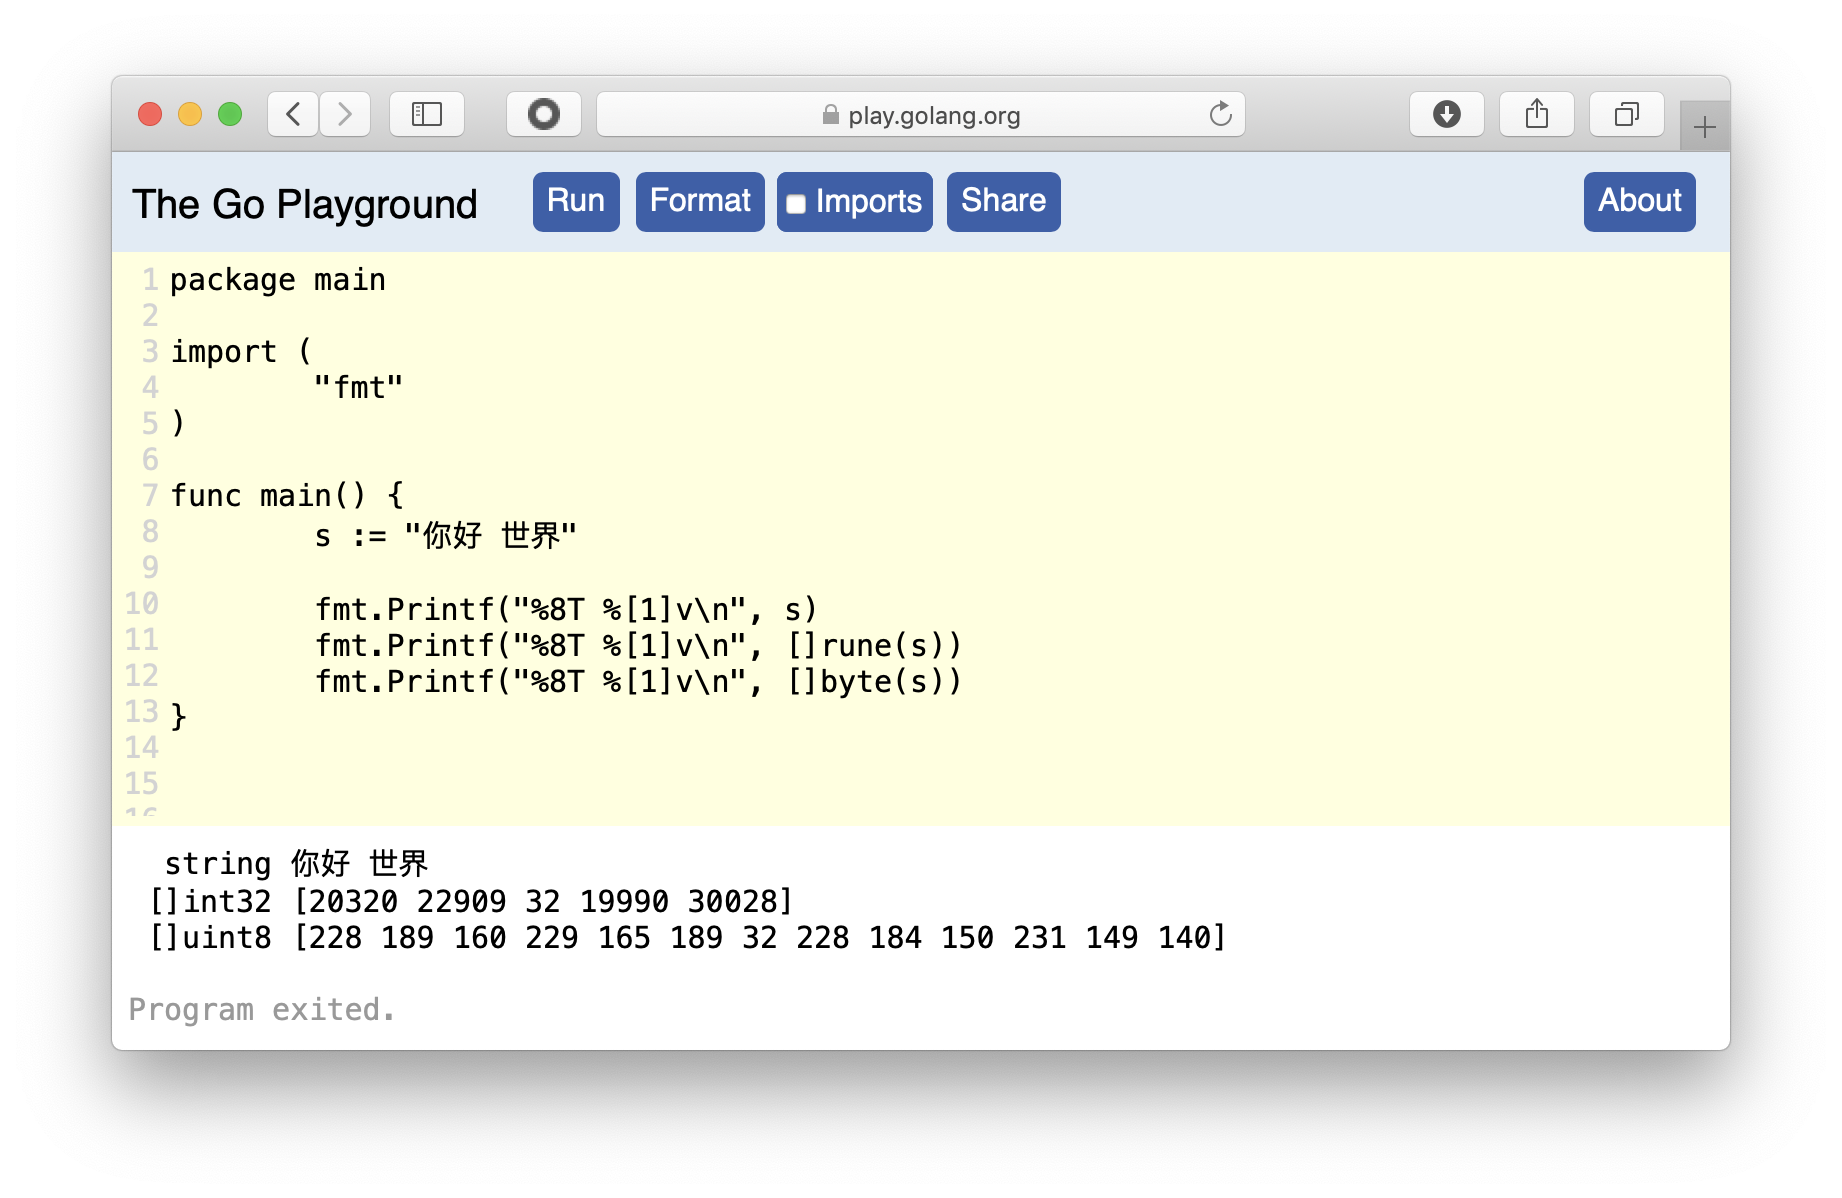
\includegraphics[height=0.9\textheight]{go-playground-chinese.png}
\end{center}
\end{frame}

\begin{frame}[fragile]
    \frametitle{Simple types}
    Special types:
    \begin{itemize}
        \item \verb|bool| (boolean) has two values \verb|false|, \verb|true| \\
        \vspace{0.5\baselineskip}
        these values are {\bf not} convertible to/from integers!
        \vspace{\baselineskip}
        \item \verb|error|: an interface type with one function \\
        \vspace{0.5\baselineskip}
        \verb|func (e *error) Error() string| \\
        \vspace{0.5\baselineskip}
        an \verb|error| may be nil or non-nil
        \vspace{\baselineskip}
        \item Pointers are physically addresses, logically opaque \\
        \vspace{0.5\baselineskip}
        a pointer may be nil or non-nil \\
        {\em no pointer manipulation} except through package \verb|unsafe|
    \end{itemize}
\end{frame}

\begin{frame}[fragile]
    \frametitle{Numeric literals}
    Go keeps ``arbitrary'' precision for literal values (at least 256 bits)
    \begin{itemize}
        \item Integer literals are untyped \\
        \begin{itemize}
        \item assign a literal to any size integer without conversion \\
        \item assign an integer literal to float, complex also
        \end{itemize}
        \vspace{\baselineskip}
        \item Ditto float and complex; picked by syntax of the literal
        \vspace{\baselineskip}
        \item Mathematical constants can be very precise \\
        {\tiny\verb|Pi  = 3.14159265358979323846264338327950288419716939937510582097494459|} \par
        \vspace{\baselineskip}
        \item Constant arithmetic done at compile time doesn't lose precision
    \end{itemize}
\end{frame}

\begin{frame}[fragile]
    \frametitle{Constants}
    Only numbers and strings can be constants \par
    \vspace{0.5\baselineskip}
    Constant can be a literal or a compile-time function of a constant
\begin{golang}
    const (
        a = 1                 // int
        b = 2 * 1024          // 2048
        c = b << 3            // 16384

        g uint8 = 0x07        // 7
        h uint8 = g & 0x03    // 3

        s = "a string"
        t = len(s)            // 8
        u = s[2:]             // SYNTAX ERROR
    )
\end{golang}
\end{frame}

\begin{frame}[fragile]
    \frametitle{Declaration}
    There are six ways to introduce a name:
    \begin{itemize}
        \item Constant declaration with \verb|const| \\
        \vspace{0.5\baselineskip}
        \item Type declaration with \verb|type| \\
        \vspace{0.5\baselineskip}
        \item Variable declaration with \verb|var| \\
        (must have type or initial value, sometimes both)
        \vspace{0.5\baselineskip}
        \item Short, initialized variable declaration of any type \verb|:=| \\
         {\em only inside a function} \\
        \vspace{0.5\baselineskip}
        \item Declaration of a function at package level with \verb|func| \\
        (methods may {\em only} be declared at package level)
        \vspace{0.5\baselineskip}
        \item Formal parameters and named returns of a function
    \end{itemize}
\end{frame}

\begin{frame}[fragile]
    \frametitle{Initialization}
    Go initializes all variables to ``zero'' by default if you don't:
    \begin{itemize}
        \item All numerical types get \verb|0| (float \verb|0.0|, complex \verb|0i|) \\
        \vspace{0.5\baselineskip}
        \item \verb|bool| gets \verb|false| \\
        \vspace{0.5\baselineskip}
        \item \verb|string| gets \verb|""| (the empty string, length 0)\\
        \vspace{0.5\baselineskip}
        \item Everything else gets \verb|nil| :\\
        \begin{itemize}
        \item pointers
        \item slices
        \item maps
        \item channels
        \item functions (function variables)
        \item interfaces
        \end{itemize}
        \vspace{0.5\baselineskip}
        \item For aggregate types, all members get their ``zero'' values \\
    \end{itemize}
\end{frame}

\begin{frame}[fragile]
    \frametitle{Examples}
\begin{golang}
// x and y get the values passed in by the caller
// the (unnamed) return value gets the "return" expression

func do(x, y int) int {
    const t = 21            // type int by default
    const z = false         // type bool from the value

    var i uint8 = 255       // explicit type uint8
    var j = 256             // type int by default
    var k int               // 0 by default

    var m                   // SYNTAX ERROR, no type/value

    j := 0                  // short declaration, int
    v := func() { ... }     // short declaration, function

    return k
}
\end{golang}
\end{frame}

\begin{frame}[fragile]
    \frametitle{Examples}
\begin{golang}
// explicit conversion is required for integer types
// and inc-/decrement operators can't be expressions

func do(x, y int) int {
    k := x + y              // k int
    m := uint32(k)          // int conversion

    k = m                   // TYPE MISMATCH

    var i uint8 = 255

    j := i++                // SYNTAX ERROR
    --i                     // SYNTAX ERROR

    b := k = 0              // SYNTAX ERROR

    return m                // TYPE MISMATCH
}
\end{golang}
\end{frame}

\begin{frame}[fragile]
    \frametitle{Basic operators}
    Arithmetic: numbers only except \verb|+| on string
{\scriptsize\begin{verbatim}
    +    -    *    /    %    ++     --
\end{verbatim}}
    Comparison: only numbers/strings support order
{\scriptsize\begin{verbatim}
    ==   !=   <    >    <=   >=
\end{verbatim}}
    Boolean: only booleans, with shortcut evaluation
{\scriptsize\begin{verbatim}
    !    &&   ||
\end{verbatim}}
    Bitwise: operate on integers
{\scriptsize\begin{verbatim}
    &    |    ^    <<   >>   &^
\end{verbatim}}
    Assignment: as above for binary operations
{\scriptsize\begin{verbatim}
    =    +=   -=   *=   /=   %=
    &=   |=   ^=   <<=  >>=  &^=
\end{verbatim}}
\end{frame}

\begin{frame}[fragile]
    \frametitle{Operator gotchas}
    The division operator \verb|/| has two meanings
\begin{golang}
    i := 3/2          // integer division
    fmt.Println(i)    // 1

    j := 51/25
    fmt.Println(j)    // 2

    t := 3.0/2.0      // real division
    fmt.Println(t)    // 1.5
\end{golang}
    \vspace{3\baselineskip}
    Aside: why are i, j, and k often used as loop index variables? \par
    \vspace{0.2\baselineskip}
    They were integer variables by default in Fortran (names i--n)
\end{frame}

\begin{frame}[fragile]
    \frametitle{Operator precedence}
    There are only five levels of precedence, otherwise left-to-right: \par
    \vspace{0.5\baselineskip}
    Operators like multiplication: 
{\scriptsize\begin{verbatim}
    *    /    %    <<   >>   &    &^
\end{verbatim}}
    Operators like addition:
{\scriptsize\begin{verbatim}
    +    -    |    ^
\end{verbatim}}
    Comparison operators:
{\scriptsize\begin{verbatim}
    ==   !=   <    <=   >    >=
\end{verbatim}}
    Logical and:
{\scriptsize\begin{verbatim}
    &&
\end{verbatim}}
    Logical or:
{\scriptsize\begin{verbatim}
    ||
\end{verbatim}}
\end{frame}

\begin{frame}[fragile]
    \frametitle{Examples}
\begin{golang}
// function has been called with x=1, y=2

func do(x, y int) int {
    k := 3 * x + y          // 5  by precedence
    m := 3 * (x + y)        // 9
    n := 3 * 5 * x + y      // 17
    p := 3 * (5 * x) + y    // 17
    v := 3 + 5 * x + y      // 10 by precedence
    w := (3 + 5) * x + y    // 10
    z := 3 + 5 * (x + y)    // 18

    b := n < 3 || p > 5     // true (2nd clause)
    c := n > 5 || z < 9     // true (1st clause)

    return k
}
\end{golang}
\end{frame}

\begin{frame}[fragile]
    \frametitle{Examples}
\begin{golang}
// function has been called with x=1, y=2

func do(x, y byte) byte {
	t := x & y              // 0
	u := x | y              // 3
	v := x &^ y             // 1
	w := ^y                 // 253
	z := x << y             // 4

    a := uint8(255)         // else signed

    a++                     // 0
    a--                     // 255

    b := x || y             // SYNTAX ERROR

    return 42               // ok, literal
}
\end{golang}
\end{frame}

%% =================================================================================

\section{Composite Types}

\begin{frame}[fragile]
    \frametitle{Strings}
    Strings are a sequence of characters and are {\bf immutable} \par
    \vspace{0.3\baselineskip}
    The built-in \verb|len| function calculates the length \par
    \vspace{0.3\baselineskip}
    Strings overload the addition operator (\verb|+| and \verb|+=|) \par
\begin{golang}
    s := "the quick brown fox"
    
    a := len(s)                   // 19
    b := s[:3]                    // "the"
    c := s[4:9]                   // "quick"
    d := s[:4] + "slow" + s[9:]   // replaces "quick"
    
    s[5] = 'a'                    // SYNTAX ERROR
    s += "es"                     // now plural (copied)
\end{golang}
    \vspace{0.3\baselineskip}
    Strings are passed {\em by reference}, thus they aren't copied
\end{frame}

\begin{frame}[fragile]
    \frametitle{String functions}
    Package \verb|strings| has many functions on strings
\begin{golang}
s := "a string"

x := len(s)                 // built-in, = 8

strings.Contains(s, "g")    // returns true
strings.Contains(s, "x")    // returns false

strings.HasPrefix(s, "a")   // returns true
strings.ToUpper(s)          // returns "A STRING"
\end{golang}
\vspace{1.5\baselineskip}
Indexes in strings are numbered from \verb|0| up to \verb|len(s) - 1|
\begin{golang}
strings.Index(s, "string")  // returns 2
\end{golang}
\end{frame}

\begin{frame}[fragile]
    \frametitle{Arrays}
    Arrays are typed by size, which is {\em fixed} at compile time
\begin{golang}
    // all these are equivalent

    var a [3]int
    var b [3]int{0, 0, 0}
    var c [...]{0, 0, 0}   // sized by initializer
    
    var d [3]int
    d = b                  // elements copied

    var m [...]int{1, 2, 3, 4}

    c = m                  // TYPE MISMATCH
\end{golang}
    \vspace{\baselineskip}
    Arrays are passed {\em by value}, thus elements are copied
\end{frame}

\begin{frame}[fragile]
    \frametitle{Slices}
    Slices have variable length, backed by some array; they are
    copied when they outgrow that array
\begin{golang}
    var a []int             // nil, no storage
    var b = []int{}         // empty but non-nil
    var c = []int{1, 2}     // non-empty

    a = append(a, 1)        // append to nil OK
    len(a), cap(a)          // 2, 2

	d := make([]int, 5)
	e := make([]int, 0, 5)  // capacity but empty

    len(d), cap(d)          // 5, 5
    len(e), cap(e)          // 0, 5
\end{golang}
    \vspace{\baselineskip}
    Slices are passed {\em by reference;} no copying, updating OK
\end{frame}

\begin{frame}[fragile]
    \frametitle{Slices}
\begin{golang}
package main
import "fmt"

func main() {
	t := []byte("string")   // 0:s 1:t 2:r 3:i 4:n 5:g

	fmt.Println(len(t), t)  // 6 bytes in t
	fmt.Println(t[2])       //   1 item
	fmt.Println(t[:2])      //   2 items
	fmt.Println(t[2:])      // 6-2 items
	fmt.Println(t[3:5])     // 5-3 items
}
\end{golang}
{\small\begin{verbatim}
6 [115 116 114 105 110 103]
114
[115 116]
[114 105 110 103]
[105 110]
\end{verbatim}}
\end{frame}

\begin{frame}[fragile]
    \frametitle{Slices vs arrays}
    Most Go APIs take slices as inputs, not arrays
\begin{center}
\begin{table}[h!]
{\renewcommand{\arraystretch}{1.7}%
    \begin{tabular}{l|l}
    \textbf{Slice} & \textbf{Array} \\
    \hline
    Variable length & Length fixed at compile time  \\
    Passed by reference & Passed by value (copied) \\
    Not comparable & Comparable ({\tt ==})  \\
    Cannot be used as map key  & Can be used as map key \\
    Has {\tt copy} \& {\tt append} helpers & --- \\
    Useful as function parameters & Useful as ``pseudo'' constants \\
    \end{tabular}}
\end{table}
\end{center}
\end{frame}

\begin{frame}[fragile]
    \frametitle{Arrays as pseudo-constants}
    It can be useful to have fixed-size tables of values in
    some algorithms, treated as constant data
\begin{golang}
// from the file crypto/des/const.go in the DES package

// Used to perform an initial permutation of a 64-bit 
// input block.
var initialPermutation = [64]byte{
	6, 14, 22, 30, 38, 46, 54, 62,
	4, 12, 20, 28, 36, 44, 52, 60,
	2, 10, 18, 26, 34, 42, 50, 58,
	0,  8, 16, 24, 32, 40, 48, 56,
	7, 15, 23, 31, 39, 47, 55, 63,
	5, 13, 21, 29, 37, 45, 53, 61,
	3, 11, 19, 27, 35, 43, 51, 59,
	1,  9, 17, 25, 33, 41, 49, 57,
}
\end{golang}
\end{frame}

\begin{frame}[fragile]
    \frametitle{The off-by-one bug}
    Slices are indexed like \verb|[1:3]| \par
    (read as the starting element and {\em one past} the ending element,
    so\\ this way we have $3-1 = 2$ elements in our slice) \par
    \vspace\baselineskip}
    For loops work the same way in most cases:
    \begin{golang}
    for i := 1; i < 5; i++ {  // in math written [1, 5)
        . . .
    }
    \end{golang}
\vspace{-0.2\baselineskip}
\begin{center}
    
\includegraphics[height=.25\textheight]{fencepost-error.png}
\end{center}
\vspace{-1.1\baselineskip}
\hspace{0.72in}{\tiny Read it on Wikipedia \href{https://en.wikipedia.org/wiki/Off-by-one_error}{OB1}}
\end{frame}

\begin{frame}[fragile]
    \frametitle{Examples}
\begin{golang}
var w = [...]int{1, 2, 3}   // array of len(3)
var x = []int{0, 0, 0}      // slice of len(3)

func do(a [3]int, b []int) []int {
    a = b                   // SYNTAX ERROR
    a[0] = 4                // w unchanged
    b[0] = 3                // x changed

    c := make([]int, 5)     // len/cap 5
    c[4] = 42
    copy(c, b)              // copies only 3 elts
    b = append(b, c...)     // reallocates!
    return c
}

y := do(w, x)
fmt.Println(w, x, y)        // [1 2 3] [3 0 0] [3 0 0 0 42]
\end{golang}
\end{frame}

\begin{frame}[fragile]
    \frametitle{Maps}
    Maps are dictionaries: indexed by key, returning a value \par
    \vspace{0.3\baselineskip}
    You can read from a nil map, but inserting will panic 
\begin{golang}
    var m map[string]int        // nil, no storage
    p := make(map[string]int)   // non-nil but empty

    a := m["the"]               // returns 0
    m["and"] = 1                // PANIC
    m = p
    m["and"]++                  // OK, same map as p now
    c := p["and"]               // returns 1
\end{golang}
    \vspace{\baselineskip}
    Maps are passed {\em by reference;} no copying, updating OK \par
    \vspace{0.3\baselineskip}
    The type used for the key must have \verb|==| and \verb|!=| defined \\
    {\em not slices, maps, or functions} \par
\end{frame}

\begin{frame}[fragile]
    \frametitle{Maps}
    Maps can't be compared to one another; maps can be compared only to
     \verb|nil| as a special case
\begin{golang}
    var m  = map[string]int{
        "and": 1,
        "the": 1,
        "or":  2,
    }

    var n map[string]int
    
    b := m == n                 // SYNTAX ERROR
    c := n == nil               // true
    d := len(m)                 // 3
    e := cap(m)                 // TYPE MISMATCH
\end{golang}
    \vspace{0.5\baselineskip}
\end{frame}

\begin{frame}[fragile]
    \frametitle{Maps}
    Maps have a special two-result lookup function \par
    \vspace{0.3\baselineskip}
    The second variable tells you if they key was there
    \vspace{0.3\baselineskip}
\begin{golang}
    p := map[string]int{}       // non-nil but empty

    a := p["the"]               // returns 0
    b, ok := p["and"]           // 0, false

    p["the"]++

    c, ok := p["the"]           // 1, true

    if w, ok := p["the"]; ok {
        // we know w is not the default value
        . . .
    }
\end{golang}
\end{frame}

\begin{frame}[fragile]
    \frametitle{Make nil useful}
    Nil is a type of zero: it indicates the absence of something \par
    \vspace{0.2\baselineskip}
    Many built-ins are safe: \verb|len|, \verb|cap|, \verb|range| \par
    \vspace{0.4\baselineskip}
\begin{golang}
    // nil -- no options
    jar, err := cookiejar.New(nil)

    // nil function -- use the default
    http.ListenAndServe("localhost:8080", nil)

    // nil []int slice -- skip the loop
    for _, v := range values {
        total += v
    }
\end{golang}
\vspace{0.6\baselineskip}
``Make the zero value useful.'' --- Rob Pike \par
\vspace{-0.4\baselineskip}
{\scriptsize See Francesc Campoy's video at \href{https://www.youtube.com/watch?v=ynoY2xz-F8s}%
{https://www.youtube.com/watch?v=ynoY2xz-F8s}}
\end{frame}

\begin{frame}[fragile]
    \frametitle{Built-ins}
    Each type has certain built-in functions \par
    \vspace{0.5\baselineskip}
{\scriptsize\begin{verbatim}
len(s)           string  string length

len(a), cap(a)   array   array length, capacity (constant)

make(T, x)       slice   slice of type T with length x and capacity x
make(T, x, y)    slice   slice of type T with length x and capacity y

copy(c, d)       slice   copy from d to c; # = min of the two lengths
c=append(c, d)   slice   append d to c and return a new slice result

len(s), cap(s)   slice   slice length and capacity

make(T)          map     map of type T
make(T, x)       map     map of type T with space hint for x elements

delete(m, k)     map     delete key k (if present, else no change)

len(m)           map     map length
\end{verbatim}}
\end{frame}

%% =================================================================================

\section{Control Structures}

\begin{frame}[fragile]
    \frametitle{Sequence}
    The simplest type of program has no ``structures'' \par
    \vspace{0.5\baselineskip}
    It just flows from top to bottom, executing statements in sequence
\begin{golang}
package main
import (
    "fmt" 
    "math"
)

func main() {
    a, b, c := -0.5, 0.5, 5.0
    x := math.Sqrt(b*b - 4*a*c) / (2 * a)
    y1, y2 := -b + x, -b - x
    
    fmt.Printf("%5.4f, %5.4f\n", y1, y2)
    // -3.7016, 2.7016
}

\end{golang}
\end{frame}

\begin{frame}[fragile]
    \frametitle{If-then-else}
    The next type of structure is a choice between alternatives \par
    \vspace{0.5\baselineskip}
    All if-then statements require braces
\begin{golang}
    if a == b {
        fmt.Println("a equals b")
    } else {
        fmt.Println("a is not equal to b")
    }
\end{golang}
    \vspace{0.5\baselineskip}
    They can start with a short declaration or statement
\begin{golang}
    if err := doSomething(); err != nil {
        return err
    }
\end{golang}
\end{frame}

\begin{frame}[fragile]
    \frametitle{Switch}
    A switch is another choice between alternatives \par
    \vspace{0.5\baselineskip}
    It is a shortcut replacing a series of if-then statements
\begin{golang}
    switch a := f.Get(); a {
    case 0, 1, 2:
        fmt.Println("underflow possible")

    case 3, 4, 5, 6, 7, 8:

    default:
        fmt.Println("warning: overload") 
    }
\end{golang}
    \vspace{\baselineskip}
    Alternatives may be empty and {\bf do not fall through} (as in C) \\
    so a \verb|break| is not required
\end{frame}

\begin{frame}[fragile]
    \frametitle{Switch on true}
    Arbitrary comparisons may be made for an switch with no argument \par
\begin{golang}
    a := f.Get()

    switch {
    case a <= 2:
        fmt.Println("underflow possible")

    case a <= 8:
        // evaluated in order

    default:
        fmt.Println("warning: overload") 
    }
\end{golang}
\end{frame}

\begin{frame}[fragile]
    \frametitle{For loops}
    The loop control structure provides automatic repetition \par
    \vspace{0.5\baselineskip}
    There is only \verb|for| (no \verb|do| or \:\verb|while|) but with options \par
    \vspace{\baselineskip}
    1. Explicit control with an index variable
\begin{golang}
    for i := 0; i < 10; i++ {
        fmt.Printf("(%d, %d)\n", i, i*i)
    }

    // prints (0, 0) up to (9, 81)
\end{golang}
    \vspace{0.5\baselineskip}
    Three parts, all optional (initialize, check, increment) \par
    \vspace{0.5\baselineskip}
    The loop ends when the explict check fails (e.g., \verb|i == 10|)
\end{frame}

\begin{frame}[fragile]
    \frametitle{For loops}
    2. Implicit control through the \verb|range| operator for arrays, \\
    slices, and maps (among others)
\begin{golang}
    // one var: i is an index 0, 1, 2, ...

    for i := range anArray {
        fmt.Println(i, anArray[i])
    }

    // two vars: i is the index, v is a value

    for i, v := range anArray {
        fmt.Println(i, v)
    }
\end{golang}
    \vspace{0.5\baselineskip}
    The loop ends when the range is exhausted
\end{frame}

\begin{frame}[fragile]
    \frametitle{For loops}
    3. An infinite loop with an explicit \verb|break|
\begin{golang}
    i, j := 0, 3

    // this loop must be made to stop

    for {
        i, j = i + 50, j * j
        
        fmt.Println(i, j)

        if j > i {
            break       // when i = 150, j = 6561
        }
    }
\end{golang}
    \vspace{0.5\baselineskip}
    There is also \verb|continue| to make an iteration start over
\end{frame}

\begin{frame}[fragile]
    \frametitle{For loops}
    Here's a {\bf common mistake} \par
    \vspace{0.5\baselineskip}
    If you only want \verb|range| values, you need the blank identifier:
\begin{golang}
    // two vars: _ is the index (ignored), 
    // v is a value

    for _, v := range anArray {
        fmt.Println(v)
    }
\end{golang}
    \vspace{1.5\baselineskip}
    Sometimes you may get a compile error for a type mismatch \par
    \vspace{\baselineskip}
    The \verb|_| is an untyped, reusable ``variable'' placeholder \par
\end{frame}

%% ================================================================================

\section{Input/Output}
\begin{frame}[fragile]
    \frametitle{Standard I/O}
    Unix has the notion of three standard I/O streams \par
    \vspace{0.5\baselineskip}
    They're open by default in every program \par
    \vspace{0.5\baselineskip}
    Most modern programming languages have followed this convention:
    \begin{itemize}
    \item Standard input
    \item Standard output
    \item Standard error (output)
    \end{itemize}
    \vspace{\baselineskip}
    These are normally mapped to the console/terminal but can \\
    be {\em redirected} \par
    {\scriptsize \verb@find . -name '*.go' | xargs grep -n "rintf" > print.txt@}
\end{frame}

\begin{frame}[fragile]
    \frametitle{Formatted I/O}
    We've been using the \verb|fmt| package to do I/O \par
    \vspace{0.5\baselineskip}
    By default, we've been printing to standard output \par
\begin{golang}
package main

import (
    "fmt"
    "os"
)

func main() {
    fmt.Println("printing a line to standard output")

    fmt.Fprintln(os.Stderr, "printing to error output")
}
\end{golang}
\end{frame}

\begin{frame}[fragile]
\frametitle{Printing command-line arguments}
\begin{golang}
package main

import "fmt"
import "os"

func main() {
    var s, sep string

    for i := 1; i < len(os.Args); i++ {
        s += sep + os.Args[i]
        sep = " "
    }

    fmt.Println(s)
}
\end{golang}
We'll skip \verb|os.Arg[0]| because that's the program name:
{\tiny \verb|/var/folders/6y/q8z5w4xn1dzb0_qz680mcs6h0000gn/T/go-build451715571/b001/exe/hello|}
\end{frame}

\begin{frame}[fragile]
    \frametitle{A whole family of functions}
    The \verb|fmt| package uses reflection and can print anything; \\
    some of the functions take a {\em format string}
\begin{golang}
// always os.Stdout

fmt.Println(...interface{}) (int, error)
fmt.Printf(string, ...interface{}) (int, error)

// print to anything that has the correct Write() method

fmt.Fprintln(io.Writer, ...interface{}) (int, error)
fmt.Fprintf(io.Writer, string, ...interface{}) (int, error)

// return a string

fmt.Sprintln(...interface{}) string
fmt.Sprintf(string, ...interface{}) string
\end{golang}
\end{frame}

\begin{frame}[fragile]
    \frametitle{Format codes}
    The \verb|fmt| package uses format codes reminiscent of C
{\scriptsize\begin{verbatim}
%s   the uninterpreted bytes of the string or slice
%q   a double-quoted string safely escaped with Go syntax
%c   the character represented by the corresponding Unicode code point

%d   base 10
%x   base 16, with lower-case letters for a-f
%f   decimal point but no exponent, e.g. 123.456
%t   the word true or false

%v   the value in a default format
     when printing structs, the plus flag (%+v) adds field names

%#v  a Go-syntax representation of the value
%T   a Go-syntax representation of the type of the value

%%   a literal percent sign; consumes no value [escape]
\end{verbatim}}
Read the godoc, Luke: \href{https://golang.org/pkg/fmt/}{https://golang.org/pkg/fmt/}
\end{frame}

\begin{frame}[fragile]
    \frametitle{Format code examples}
    \verb|%#v| and \verb|%T| are very useful for describing what something is:
\begin{golang}
a := []int{1, 2, 3}
b := [3]rune{'a', 'b', 'c'}
p := map[string]int{"and":1, "or":2}

fmt.Printf("%T\n", a)   // []int
fmt.Printf("%v\n", a)   // [1 2 3]
fmt.Printf("%#v\n", a)  // []int{1, 2, 3}

fmt.Printf("%T\n", b)   // [3]int32
fmt.Printf("%q\n", b)   // ['a' 'b' 'c']
fmt.Printf("%v\n", b)   // [97 98 99]
fmt.Printf("%#v\n", b)  // [3]int32{97, 98, 99}

fmt.Printf("%T\n", p)   // map[string]int
fmt.Printf("%v\n", p)   // map[and:1 or:2]
fmt.Printf("%#v\n", p)  // map[string]int{"and":1, "or":2}
\end{golang}
\end{frame}

\begin{frame}[fragile]
    \frametitle{Reading a file}
    Here's another program that checks a file's size
\begin{golang}
package main

import ("fmt"; "io/ioutil"; "os")

func main() {
    fname := os.Args[1]
    if f, err := os.Open(fname); err != nil {
        fmt.Fprintln(os.Stderr, "bad file:", err)
    } else if d, err := ioutil.ReadAll(f); err != nil {
        fmt.Fprintln(os.Stderr, "can't read:", err)
    } else {
        fmt.Printf("The file has %d bytes\n", len(d))
    }
}
\end{golang}
If run on itself (the source file), it prints ``The file has 333 bytes''
\end{frame}

\begin{frame}[fragile]
    \frametitle{Reading a file}
    Wait, what's going on here?
\begin{golang}
if f, err := os.Open(fname); err != nil {
    fmt.Fprintln(os.Stderr, "bad file:", err)
} . . .
\end{golang}
    \vspace{0.5\baselineskip}
An if-statement can have a short declaration as its first part \par
    \vspace{\baselineskip}
We often call functions whose 2nd return value is a possible error \par
\begin{golang}
    func Open(name string) (*File, error)
\end{golang}
where the \verb|error| can be compared to \verb|nil|, meaning no error \par
    \vspace{\baselineskip}
\alert{\bf Always check the error} --- the file might not really be open! \par
\end{frame}


%% ================================================================================

\section{Homework}
\begin{frame}[fragile]
    \frametitle{Homework \# 1}
    Write a program to take a list of files from the command line \\
    and count the words in them. A word is anything separated by whitespace 
    (so detached punctuation will count). \par
    \vspace{0.5\baselineskip}
    You can test your first program with \verb|wc|: \par
    {\scriptsize
\begin{verbatim}
  $ wc testing.txt
         9      35     180 testing.txt
\end{verbatim}} \par
    \vspace{0.5\baselineskip}
    Then create an option to count only {\em unique} words. \\
    You can test this with: \par
    {\scriptsize
\begin{verbatim}
  $ awk '{for (i=1;i<=NF;i++) {print $i}}' testing.txt|sort|uniq|wc
        26      26     144
\end{verbatim}} \par
    \vspace{0.5\baselineskip}
    You may want to use \verb|ioutil.ReadFile| and \verb|strings.Fields|
\end{frame}

\end{document}